\chapter{Veränderungsprozesse in Organisationen}
Dieses Kapitel analysiert die Einflüsse aus den Rahmenbedingungen für Veränderungsprozesse der Institute und trägt kontinuierlich zur Findung der Ursachen der genannten Probleme und Ansätze für ihre Lösung bei. Der \emph{Design-Thinking} Prozess wird hierbei als iterative Innovationsmethode für Ideen, Prototypen und kontinuierlicher Evaluierung verwendet. Daher bauen die nachfolgenden Abschnitte aufeinander auf und sollen somit zu einer kontinuierlichen Verbesserung beitragen.

\section{Innovation und Transformation}

\cite{Ganswindt2006} und \cite{Koch2016} identifizieren bereits, dass das \ac{ITM} nicht in der Lage ist die Maßnahmen für eine Transformation zu priorisieren.
Die gegenseitigen Einflüsse sind ineinander verwachsen und häufig werden zu erst die Symptome bekämpft (Anh.\ref{appendix:docker}, Kap. \ref{jenkins:skalierung}).

\paragraph{einschränkende Faktoren zusammengefasst}
\label{einschr:assets}
Aufgrund dieser Verwachsungen wird in der folgenden Auflistung eine grobe Lokalisierung der Einschränkungen vorgenommen:
\begin{itemize}
    \item \textbf{Organisation:} tiefe Silos \cite{Gupta:2017}, Schatten-IT \cite{recht/Bornemann2018}, Abhängigkeiten, Handlungsunfähigkeit, Redundanzen
    \item \textbf{IT-Architektur:} Komplexität \cite{Brockhoff2006}, steigende Anforderungen \cite{Brockhoff2006}, Kosten für Eigenentwicklung \cite{Gupta:2017}, Proprietäre Anwendungen \cite{Bussmann2006}
    \item \textbf{Regulatorik:} \ac{IDV} Katalogisierung\cite{recht/Bornemann2018}, fehlende Präzisierung, steigende Anforderungen,
\end{itemize}

\citet[Kap. 2.2]{Alt2017} erklären die Abläufe in Folge einer Innovation. Die Abbildung \cite[Abb. 2.1]{Alt2017} beschreibt einen Innovationsverlauf als eine \emph{S-Kurve} \cite{Ganswindt2006}, die in Folge mehrerer Innovationen gesamtheitlich betrachtet einen disruptiven Verlauf zeigen. Darunter liegt die Adaptionskurve, die als die Ableitung der Innovationskurve erscheint. 
\medskip
\\
Einschränkenden Faktoren, die in Banken beobachtet werden, könnten als Faktor der Adaptionskurve in \cite[Abb. 2.1]{Alt2017} zugeordnet werden. Demgegenüber stehen die zu erarbeitenden Gegenmaßnahmen zur Lösung des Problems.
\medskip
\\
Hierbei fällt auf, dass die als Faktor wahrgenommenen Einschränkungen aus den Rahmenbedingungen in diesem Kapitel zwischen Zuständen und ihren Eigenschaften unterschieden werden können. Daher sind einige Einschränkungen Rahmen, die einen Zustand enthalten. Ihre negativen Eigenschaften sind hierbei die Faktoren, welche die Adaptionskurve hemmen könnten. Es macht im ersten Blick durchaus Sinn, dass die Einführung einer innovativen Technologie 
\medskip
\\
In einem ersten Rückblick, zwischen den untersuchten Maßnahmen und dem Innovationsverlauf in \cite{Ganswindt2006, Alt2017} kann folgendes festgestellt werden.


\begin{itemize}
    \item Das Problem besteht in der \emph{Transformationsfähigkeit} eines Unternehmens. 
    \item Um diese zu steigern müssen Maßnahmen ermittelt werden, welche die Amplitude der Adaptionskurve \cite[Abb. 2.1]{Alt2017} \emph{kontinuierlich \cite{Bussmann2006}} aufrecht erhalten. 
\end{itemize}

\subsection{Prototyp zur Regelung von Innovation}

\paragraph{Innovationsverlauf}
Die Einflüsse im Zusammenhang mit Innovation könnten folgendermaßen klassifiziert werden:
\begin{enumerate}
    \item \textbf{Impulse} für einen bevorstehenden Transformationsprozess. Für Veränderung werden Impulsgeber benötigt wie zum Beispiel Technologien \cite{Bussmann2006, Gupta:2017}. Der Impuls kann als die Innovation selbst gesehen werden. Aus der Ableitung der Adaptionskurve \cite[Abb. 2.1]{Alt2017} wird deutlich, dass der Hochpunkt der Adaption mit der Auswirkung oder Effektivität der Innovation korreliert.
    \item \textbf{Auslöser} für die Klassifizierung der Innovation. Sie ist für die Entscheidung über die Maßnahmen gegenüber den Impulsen wichtig.
    \item \textbf{Parameter} für die Antizipation der \emph{bevorstehenden} Transformation. \emph{Bevorstehend} impliziert auch eine Unvermeidbarkeit, die sich aus disruptiven Eigenschaften einer Innovation ergibt \cite{Fernandez:2020, Gupta:2017}
    \item \textbf{Antriebe} als Faktoren, die die \emph{bevorstehende} Transformation begünstigen. Sie drücken möglicherweise die Innovationskraft oder Effektivität der Organisation aus.
\end{enumerate}
Die höchstmögliche Transformationsfähigkeit wäre mit der geringsten Differenz zwischen der \emph{angestrebten} Adaptionskurve \cite[Abb. 2.1]{Alt2017} und der Transformationsfähigkeit möglich.

\paragraph{Regelung der Transformation}
Veränderungen unterliegen kreativen Prozessen \cite[S.14]{Alt2017}, weswegen eine kreative Methode sich für ihr Verständnis eignen könnte. Gerade der \emph{Design-Thinking} Prozess sieht die iterative Gestaltung und Evaluierung von Prototypen vor. Dadurch können Zusammenhönge untersucht werden und der Lösungsansatz kann ständig angepasst werden.
\medskip
\\
\begin{figure}[htbp]
 \centering
 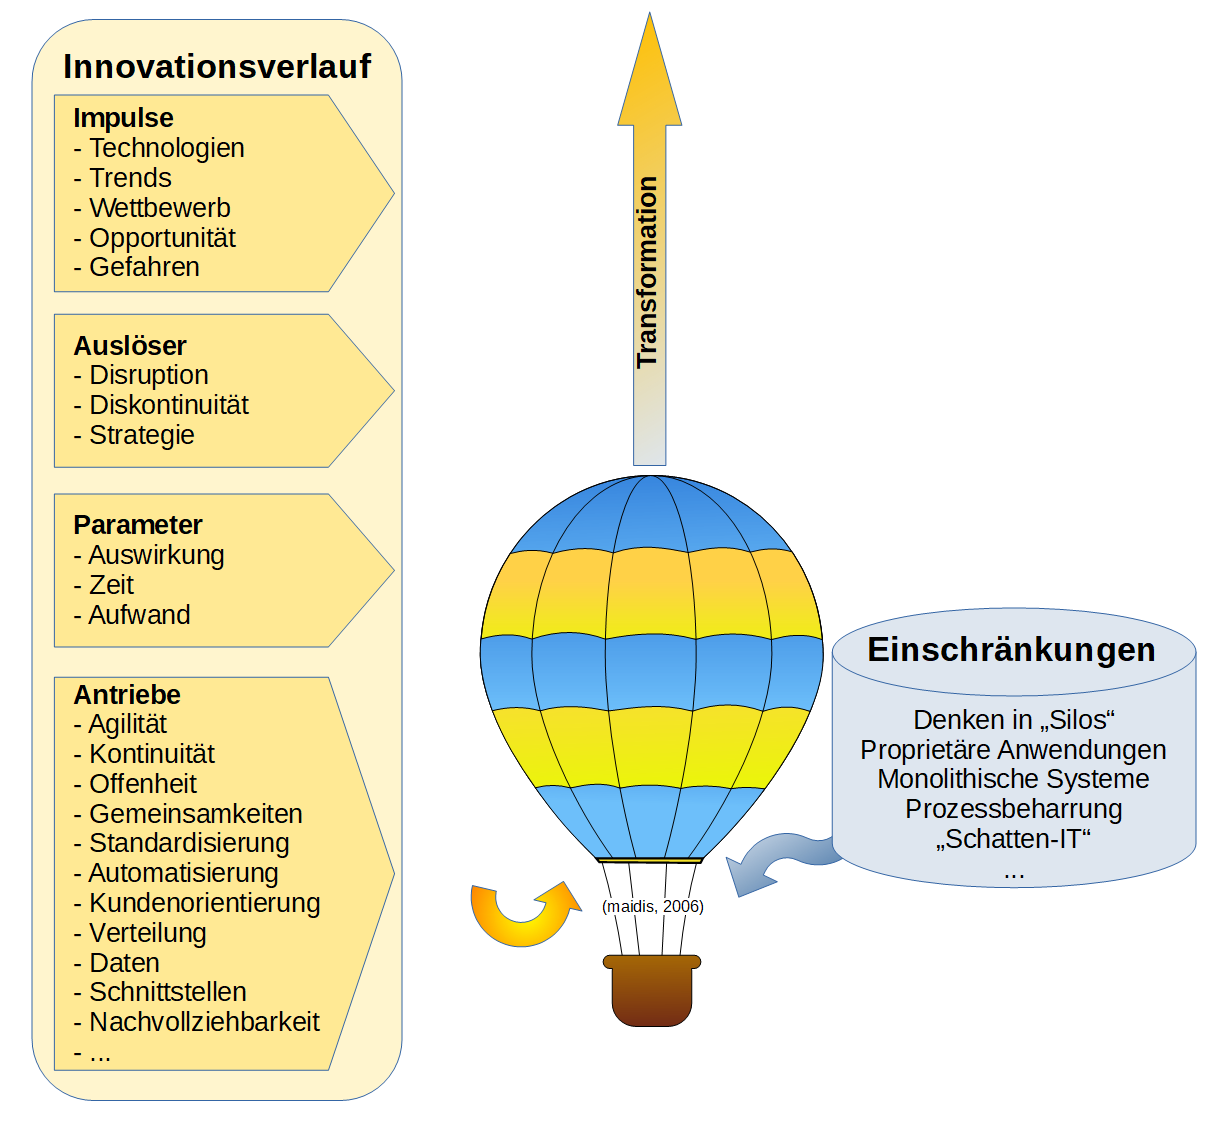
\includegraphics[width=1.0\textwidth]{gfx/digital-transformation-lifecycle-by-selim3.PNG}
 \caption{Innovationsverlauf und Regelung der Transformation (Quelle: eigene Darstellung, Heißluftballon von \citet{maidis_2006})\label{fig:digit-trans}
 }
\end{figure}
\medskip
\\
Abb. \ref{fig:digit-trans} ist aus der Zusammenfassung von antreibenden und einschränkenden Faktoren entstanden. Der Begriff der antreibenden und einschränkenden Faktoren generierte in Zusammenhang mit dem Transformationsziel der heutigen IT-Architekturen hin zu einer Cloud-Architektur die Idee von einem Heißluftballon als Metapher für die sich transformierende Organisation.

Zu antreibenden Faktoren für Veränderungen wurden weitere Kategorien aus den Ergebnissen dieses Kapitels ergänzt. Die Antriebe sind hierbei ein Soll-Zustand, der eine 

Ein Veränderungsprozesse oder Transformation beginnt nicht allein mit dem Treibstoff. Der Prozess setzt einen Funken als Auslöser voraus, um ihn zu beginnen. Dieser kann kontrolliert anhand einer Strategie gesetzt werden oder durch äußere Einflüsse unkontrolliert in Form einer Disruption oder Diskontinuität \cite{Fernandez:2020} des aktuellen Zustands.
\medskip
\\
Die Analogie eines Heißluftballon für die Regelung der Transformation kann folgendermaßen fortgeführt werden:

Die Veränderungsprozesse im Ballon sind dynamisch und bewegen mit genug Antrieb ein statisches Abbild der Organisation, welcher im Korb des Heißluftballon liegt und einen Zustand der Organisation beschreibt. Der Korb ist in sich geschlossen und beinhaltet den Ablauf und Aufbau des Kerngeschäfts. Dieser trägt zu ihrer Unterstützung viele weitere Funktionen mit, die jeweils die Bewegung der Organisation durch ihre Last exponentiell einschränken. Die Bewegung kann auf zwei Arten beschleunigt werden. Der Antrieb wird erhöht oder ein Teil der Einschränkungen abgeworfen. Sie kann nicht gesteuert werden, wodurch externe Einflüsse sie stark beeinflussen können. Das Objekt gleitet in diesem hierbei im Strom einfach mit. Beim Fliegen das Gewicht des Heißluftballon (Abb. \ref{fig:digit-trans}) eine größere Rolle wie ihr Antrieb. Mit zunehmendem Gewicht steigt der Aufwand exponentiell.
\medskip
\\
\paragraph{Lehren aus Docker}
Ein statisches Abbild mit Prozessbeschreibungen und Ausführung als eine in sich geschlossene Einheit ist aus der Virtualisierung von Systemen bekannt. Mit zunehmender Automatisierung der Geschäftsprozesse finden sich auch zunehmende Gemeinsamkeiten zwischen Organisationen und IT-Systemen. 

Best-Practices zur Beschreibung von Images mit Docker könnten als Inspiration für Organisationen dienen. Besonders das Minimalisieren von Images und Konzepte wie Kubernetes zur flexiblen Skalierung und Orchestrierung von ganzen System könnten als Idee für eine flexible und skalierbare Orchestrierung von Veränderungen für die Organisation dienen, um ihre Transformation zu automatisieren. Der schmerzvolle Rollout bei wesentlichen Veränderungen in großen Organisationen könnte in eine vollautomatisierte Orchestrierung umgewandelt werden.
Agile Prinzipien in der Kultur wären das Docker und ein neues effektives Change-Management das Kubernetes des Managements.

Nach einer solchen zukünftigen Entwicklung wäre die Idee von \emph{Development as a Service} \ref{Disruption:DaaS} mit entsprechenden eingespielten Abläufen durchaus realistisch. Andere disruptive Entwicklungen sind auch nicht ausgeschlossen. Umso wichtiger ist es einen Weg zu finden die Digitale Transformation zu beherrschen.

%
%
%
%


\paragraph{Transformationsfähigkeit als Prinzip}
Abb. \ref{fig:digit-trans} stellt für den Umgang mit wesentlichen Veränderungen ein erstes Prototyp dar. Sie impliziert, dass antreibende und einschränkende Faktoren erhebliche Einflüsse für die bevorstehende Transformation haben. Die Abbildung beschreibt möglicherweise einen Zustand vor einer bevorstehenden Transformation.

Daher dient sie als Grundlage, um Anforderungen für einen innovativen Soll-Zustand zu simulieren. Ein innovativer Soll-Zustand der Organisation würde eine höchstmögliche Transformationsfähigkeit antreiben. 
\medskip
\\
Gleichzeitig zeigt sie, dass mit Anforderungen und Kenntnissen über Einschränkungen eine bevorstehende Transformation nur geregelt werden kann und die Richtung nicht absehbar ist. Gas geben ohne zu lenken ist für FinTechs und Start-ups kein großes Problem, da aufgrund ihrer kleinen Größe die Auswirkungen von Veränderungen einfacher analysiert werden können.

Für die größeren, etablierten Institute gilt ein erhöhter Schutzbedarf \cite{recht/Bornemann2018} und dadurch zusätzliche Maßnahmen für die Kontrolle von operationellen Risiken \cite{MaRisk:2017, BAIT:2018}. Diese müssen gezwungenermaßen sich neu ausrichten \citet{Bussmann2006, Gupta:2017}, indem sie ihre hohe Masse in Bewegung versetzen. Analog impliziert es eine Unkontrollierbarkeit von möglichen Problemen und Risiken.

\subsection{Frage an das Management: Change oder Run?}
\citet[11.4.1]{Koch2016} fordern für ein Management der Transformation:
\begin{quote}
    \enquote{Erstens ist zu akzeptieren, dass der
Transformationsprozess nicht im Kontext eines einmaligen begrenzten Projektes vollzogen
werden kann. Vielmehr bedarf es einer langfristigen Initiative, damit die notwendigen
Fähigkeiten entwickelt werden können. Zweitens darf die Transformation nicht als rein
technologische Initiative interpretiert werden.}
\end{quote}

Die Entwicklung von skalierbaren und flexiblen Systemen für die \ac{SEU} von Banken setzt wesentliche Veränderungen in der IT-Architektur, Prozesse und Organisation eines Instituts voraus. Erfolgen diese nicht werden umfangreiche Anpassungen der verwendeter Standardsoftware und Abänderungen von gängigen Lösungen bedingt \ref{grundlagen:ci-in-banken}.
\medskip
\\
In folge dessen sind die Veränderungsprozesse selbst zu optimieren und die Einschränkungen hierfür zu eliminieren. Kontinuierliche Veränderungen setzen kontinuierliche Prozesse voraus (Abb. \ref{fig:devops}). Standards in der Softwareentwicklung sind agil und verändern sich ständig. Eine flexible IT-Architektur ist erforderlich, um sich diesen Veränderungen anzupassen \cite{Bussmann2006}.

\paragraph{Errichtung von Anlagen}
\label{anlagen:capabilities}
Aus Sicht der Entwicklung und Beteiligten an Change-Prozessen könnte bezüglich der Einschränkungen auf die Regulatorik oder Betrieb verwiesen werden.

Dagegen spricht aus Sicht des Betriebs, dass Change-Prozesse zuerst sich selbst zu optimieren haben und dadurch die richtigen Prioritäten setzen, bevor sie den ohnehin konservativen Betrieb optimieren. Die Skalierbarkeit und Flexibilität der IT-Architektur sollte nicht aufgrund ihrer Symptome gefordert werden, sondern als eine Anlage\footnote{vgl. \enquote{capabilities} in \cite{Koch2016}}, um weitere Innovationen zu fördern.
\medskip
\\
Möglich wäre eine Strategie, in der Entwickler und Geschäftsleitung eng zusammenarbeiten.
Beim Durchleuchten der Einschränkungen aus verschiedenen Perspektiven fällt auf, dass die konservative Haltung des IT-Betriebs und der Regulatorik eine valide Berechtigung, gerade im Finanzwesen hat. Die Anforderungen selbst sind trotzdem flexibel gestaltet und bieten einen Ermessensspielraum. 

\paragraph{Gestaltungsmethoden für IT-Management}
Neben externe Auslöser von Innovation, die Unternehmen aufgrund von Disruption und Diskontinuität zu Veränderungen zwingen \cite{Gupta:2017, Fernandez:2020} existiert die IT-Strategie als interner Auslöser \cite{BAIT:2018, Alt2017}, dessen Verantwortung in erster Linie der Geschäftsleitung unterliegt \cite{BAIT:2018}. Daher sollten zu erst die Veränderungsprozesse optimiert werden. Eine klare IT-Strategie optimiert sich selbst bevor Forderungen gestellt werden. Dies wird durch Gestaltungsmethoden wie \emph{Design-Thinking} hervorgehoben, indem sie die Quellen zu fremden Problemen zuerst auf sich selbst richten \cite{yüksel:digit}. Gestaltungsmethoden wie Design-Thinking werden gerade für Innovationsprozesse und für das \ac{ITM} empfohlen \cite{Alt2017, Koch2016}. Zudem sollte die in \citet[AT 8.2]{MaRisk:2017} geforderte Analyse und Beteiligung bei wesentlichen Veränderungen schon in den Gestaltungsprozessen stattfinden \cite{Dorschel2018}. Eine Mitgestaltung nach agilen Methoden (Abb. \ref{fig:devops}) ist auch im IT- und Risikomanagement erforderlich, um effiziente Abläufe und Maßnahmen zu schaffen.

\paragraph{Forderung eines effektiven Veränderungsmanagements}
Für die Vorhersehbarkeit von Auswirkungen ist ein kontrollierter Umgang mit Veränderungsprozessen erfordert. Um wesentliche Veränderungen kontinuierlich zu ermöglichen muss die Analyse ihrer Auswirkungen \cite{MaRisk:2017} ebenfalls effektiv sein. Die Vorhersehbarkeit der Auswirkungen von Veränderung sollte nicht nur aufgrund der Regulatorik erfüllt werden. Sie ist als eine Voraussetzung für eine klare Sicht und Zielorientierung für die Transformation anzustreben.
\medskip
\\
Ein effektives Veränderungsmanagement hat das Ziel einen Zustand der höchstmöglichen Transformationsfähigkeit zu erreichen. Hierfür ist ein grundlegend innovatives Paradigma vonnöten. 

\paragraph{Innovativer Soll-Zustand der Kultur}
Die innovative Soll-Kultur (Abb. \ref{fig:digit-trans}, Antriebe) impliziert hierbei Qualitätsansprüche für die Ergebnisse von Innovationsprozessen.

Die Qualitätsansprüche sind Gegenmittel die einschränkenden Faktoren für Veränderung.
Sie dienen daher als Grundlage, um nach einer Kultur zu streben, die sich Transformationsfähigkeit als Prinzip setzt.

Nach \citet[S.30]{Bussmann2006} ist eine kontinuierliche Justierung für den Unternehmenserfolg wichtig. Als eine der Schwierigkeiten nennt er ein effektives Management der Veränderungsprozesse.
\medskip
\\
Diese Schwierigkeit hat sich in Banken bis heute noch bewährt.
Daher wird zum Prototyp aus Abb. \ref{fig:digit-trans} ein erweitertes Modell bedingt. Für den Umgang mit kontinuierlichen Veränderungen erfordert es effiziente kontinuierliche Veränderungsprozesse.
Damit sollen bevorstehende und unvermeidbare Transformationen der Organisation kontrollierbar stattfinden.
Die Frage zu einem Umgang mit kontinuierlichen Veränderungen betrifft das Veränderungsmanagement.
\medskip
\\
\citet[S. 184f]{Koch2016} ordnen das Veränderungsmanagement zu den wichtigsten Anforderungen an ein zukünftiges Paradigma der IT-Organisation. Das bisherige Modell \emph{Plan-Build-Run} ersetzen sie mit einem neuen Paradigma, dem \emph{Innovate-Design-Transform}.
\medskip
\\
Daher wird klar warum das Modell aus Abb. \ref{fig:digit-trans} nicht zufriedenstellend genug ist. Sie identifiziert anhand der Antreiber und Einschränkungen viele Anforderungen aus \cite[Tab. 11.1]{Koch2016} aus den Bereichen Innovations- und Gestaltungsfähigkeit. Für ein Paradigmenwechsel großer Organisationen spielt die Transformationsfähigkeit die entschiedenste Rolle.
 \paragraph{Ökologisches Veränderungsmodell: IDTA-Modell}
 \begin{figure}[htbp]
 \centering
 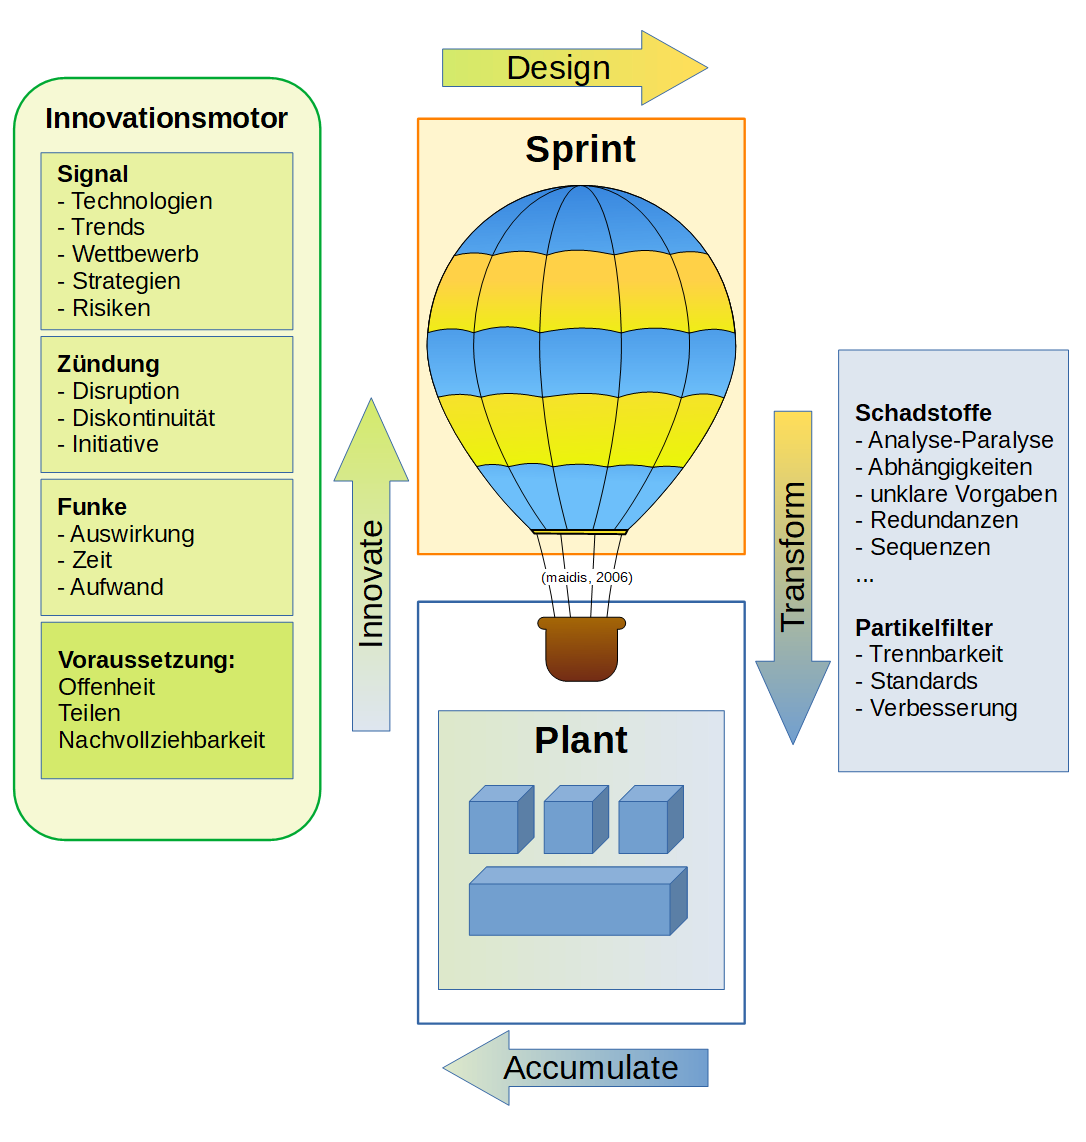
\includegraphics[width=1.0\textwidth]{gfx/digital-transformation-lifecycle-by-selim4.PNG}
 \caption{Transformations-Lebenszyklus: Kontinuierlicher Veränderungsprozess nach Innovate-Design-Transform inklusive Accumulate (Quelle: eigene Darstellung, Heißluftballon von \citet{maidis_2006})\label{fig:digit-trans-idt}
 }
 \end{figure}

In Anlehnung am DevOps Lebenszyklus \ref{fig:devops} \cite{Alt2017} wurde ein kontinuierliches Konzept für die gezielte Steuerung von Innovationsabläufen ausgearbeitet \cite{Ganswindt2006}.

Während das DevOps Lebenszyklus \cite{Alt2017} sich auf einen kontinuierlichen Prozess für die Optimierung eines IT-Produkts oder IT-Service bezieht, soll diese Abbildung \ref{fig:digit-trans} sich auf einen kontinuierlichen Prozess für die Optimierung der IT-Organisation beziehen, indem die Verbesserungsprozesse selbst in einem kontinuierlichen Prozess ihr Ergebnis ständig verbessern können.
 
\subsection{Vom Innovationsverlauf zum ökologischen Innovationsmotor}
Der für Abb. \ref{fig:digit-trans} ausgearbeitete Innovationsverlauf stellt einen ersten Zusammenhang für die schwer zu überblickenden und zu beherrschenden und Abläufe, wodurch Innovationsprozesse in Gang gesetzt werden. Die Impulse, welche die Ausgaben der schwierig zu erkennenden fremden Abläufe sind konnten dadurch grob klassifiziert werden. Das Innovationsmanagement hat zu erkennen, dass der Innovationsprozess extern bereits gestartet wird und die Ausgaben der externen Abläufe die Organisation durchdringen. Für die Beherrschbarkeit der unvermeidbaren Innovationseinflüsse hat das Innovationsmanagement sich zur Aufgabe machen die externen Impulse wahrzunehmen und die Abläufe abzufangen und gegebenenfalls zu übernehmen.
Dabei ist es von besonderer Bedeutung das Risikomanagement in diesen Überwachungsprozess mit gestalterischen Tätigkeiten miteinzubeziehen. Ein sich aufbrauender Veränderungsprozess macht sich mit kleinen Impulsen bemerktbar, bevor es disruptiv in die Athmosphäre der Organisation eindringt. Die Gefahr der Disruption muss mitigiert werden, indem die Innovation gekapert wird. 
\medskip
\\
Das Risikomanagement hat eine parallele Einheit zu errichten, die sich nicht als Ordnungsbehörde mit Strafzetteln in Form von Moniten sieht, sondern gegen Disruption als taktische Einheit aggressiv in Form von Mitgestaltung und Initiative vorgeht.
\medskip
\\
\citet{Fernandez:2020} sieht Disruption von Technologien ebenfalls als Angriff auf die Organisation. Das gleiche zeigt sich in der Korrespondenz zu den EBA-Richtlinien \cite{eba:2019}. Die \ac{BaFin} sollte die Gefahr der Disruption ebenfalls erkennen und eine klare Anforderung an die IT-Strategie und Risikomanagement zur Erhaltung der Transformationsfähigkeit des Unternehmens mit innovationsorientierten Einheiten stellen.
Daher hat die Gestaltung des Innovationsmanagements Implikationen auf das Risikomanagement. Die Aufsicht sieht den Begriff Innovation oder Disruption in \cite{MaRisk:2017} und \cite{BAIT:2018} nicht vor. Sie fordert in \cite{BAIT:2018} jedoch eine IT-Strategie, dass einige Ausgangsvariablen\footnote{In diesem Kapitel als Faktoren für Veränderung grob eingeführt} von Innovationsabläufen beinhaltet. 
Disruptive Technologien greifen den Markt an \cite{Fernandez:2020} und somit auch das Geschäftsmodell der etablierten Institute (\ref{Disruption:Blockchain}) und sind daher ein operationelles Risiko. Diese Tatsache ist seit längerem bekannt \cite{Ganswindt2006} und wird nicht berücksichtigt.
\medskip
\\
Aufgrund der Risikosituation in Zeiten der Digitalen Transformation wird zu den \ac{MaRisk} \cite{MaRisk:2017} im Rahmen der Ermessensfreiheit der Institute folgende Maßnahmen gefordert:
\begin{enumerate}
    \item Die Geschäftsleitung hat in der Gestaltung der Geschäftsstrategie die IT-Strategie als Kernkompetenz einzubeziehen
    \item Die IT-Strategie hat die Transformationsfähigkeit des Instituts sicherzustellen und Innovationsprozesse kontinuierlich zu verbessern
    \item Das Risikomanagement ist in das Innovationsmanagement einzubeziehen
    \item Das Risikomanagement hat Impulse aus Innovationsverläufen zu überwachen und gegen Disruptionen ein Notfallkonzept für Transformationsprozesse auszuarbeiten. Insbesondere hat sie die Aufgabe eine Disruption zu erkennen und eine Transformation aktiv vorzubereiten.
\end{enumerate}